\section{Поточечная и равномерная сходимость последовательности функций. Определение и примеры. Критерий равномерной сходимости. Следствия}

\begin{conj}
    Поточечная сходимость.

    Пусть $f_n, f: E \to \R$. 
    Тогда говорят, что $f_n$ поточечно сходится к $f$, если \[ \forall x \in E \; \lim_{n \to +\infty} f_n(x) = f(x) \]
    Обозначение: $f_n \to f$,  где $f$ -- предельная функция.
\end{conj}

То есть смысл такой, что мы фиксируем конкретный $x_0$, подставляем его во все функции, получаем обычную числовую последовательность, находим ее предел и говорим,
что это $f(x_0)$.
Проделываем это для всех $x_0 \in E$ и получаем $f$, заданную на $E$.

\vspace*{5mm}

\begin{conj}
    Равномерная сходимость.

    Пусть $f_n, f: E \to \R$.
    Тогда говорят, что $f_n$ равномерно сходится к $f$ на $E$, если \[ \forall \; \varepsilon > 0 \; \exists N: \; \forall n \geqslant N \; \forall x \in E \; \abs{f_n(x) - f(x)} < \varepsilon \]
    Обозначение: $f_n \doublerightarrow f$.
\end{conj}

\vspace*{5mm}

На первый взгляд определения очень похожи.
Чтобы заметить отличия, давайте запишем определение поточечной сходимости с кванторами: \[ \forall x \in E \; \forall \varepsilon > 0 \; \exists N: \forall n \geqslant N \; \abs{f_n(x) - f(x)} < \varepsilon \]
Теперь видим, что в определении поточечной сходимости $N$ выбирается для каждого $x \in E$ по отдельности, 
в то время как в определении равномерной сходимости выбирается универсальное $N$, подходящее для всех $x \in E$.

Заметим, что условие равномерной сходимости более сильное, и в частности, $f_n \doublerightarrow f \Longrightarrow f_n \to f$.
Приведем пример, показывающий, что обратной стрелки у нас нет.

\vspace*{5mm}

\begin{example}
    $E = (0, 1), \, f_n(x) = x^n, \, f_n \to f \equiv 0$ (при подстановке каждого $x$ в пределе получаем 0)

Запишем определение равномерной сходимости:
\[ \forall \varepsilon > 0 \; \exists N: \; \forall n \geqslant N \; \forall x \in (0, 1): \; x^n < \varepsilon \]
\end{example}
Понятно, что это неправда, ведь зафиксировав конкретный $\varepsilon < 1$ и конкретный $N$, для любого $n \geqslant N$ мы всегда сможем найти такой $x$ близкий к 1, что $x^n \geqslant \varepsilon$.
Таким образом, равномерной сходимости нет.

\vspace*{7mm}

\textbf{Поясняющая картинка к равномерной сходимости}.

Пусть $f_n \rightrightarrows f$. 
Тогда условие \[ \forall \; \varepsilon > 0 \; \exists N: \; \forall n \geqslant N \; \forall x \in E \; \abs{f_n(x) - f(x)} < \varepsilon \] 
означает, что для любого $\varepsilon > 0$ найдется такой достаточно большой номер $N$, что, начиная с него, графики всех функций $f_n(x)$ будут лежать в полоске шириной $2\varepsilon$ относительно графика $f(x)$:
\begin{center}
    %\includegraphics[scale=0.5]{Uniform_convergence.png} 
    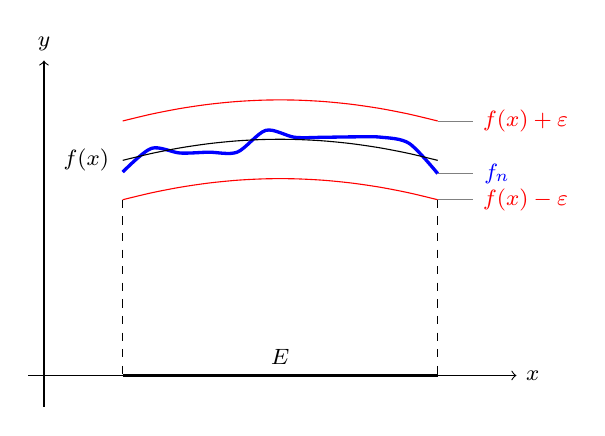
\begin{tikzpicture}[auto,
        B/.style = {decorate,
                    decoration={brace, amplitude=3pt,
                    pre=moveto,pre length=1pt,post=moveto,post length=1pt,
                    raise=1mm}},
           domain = -30:30, samples=12, smooth,
             font = \footnotesize
                                ]
        % coordinates
        \draw[->] (-0.2,0) -- (6,0) node[right]{$x$};
        \draw[->] (0,-0.4) -- (0,4) node[above]{$y$};
        % curve
        \draw[very thick, blue] 
            plot ({(45+\x)/15},{1+rand/5+2*cos(\x)})
            node[coordinate,pin=0:$f_n$] {};
        % convergence borders
        \draw[red]  plot ({(45+\x)/15},{1.5+2*cos(\x)}) 
                    node[coordinate,pin=0:$f(x)+\varepsilon$] {};
        \draw[black] plot ({(45+\x)/15},{1.0+2*cos(\x)}) coordinate (e2);
        \draw[red]  plot ({(45+\x)/15},{0.5+2*cos(\x)}) 
                    node[coordinate,pin=0:$f(x)-\varepsilon$] {};
    
        % labels on the left side
        \draw (1,{1.75+cos(-10)}) node[left=0.5mm]   {$f(x)$} ++ (0,1);
        \draw[dashed]   (1,{0.5+2*cos(30)}) -- (1,0)
                        (5,{0.5+2*cos(30)}) -- (5,0);
    
        \draw[very thick]    (1,0) -- node[above] {$E$} (5,0);
        
    \end{tikzpicture}   
\end{center}

Мы можем задать эквивалентное определение равномерной сходимости, которое на практике иногда оказывается чуть более удобным, 
хотя по сути это просто переформулировка изначального.

\begin{theorem}
    $f_n \doublerightarrow f$ на $E \Longleftrightarrow \sup\limits_{x \in E}{\abs{f_n(x) - f(x)}} \to 0$
\end{theorem}
\begin{proof} \quad

    "$\Longrightarrow$":
    \begin{gather*}
        \begin{split}
            f_n \doublerightarrow f \text{ на } E &\Longleftrightarrow \forall \varepsilon > 0 \;\; \exists N \;\; \forall n \geqslant N \;\; \forall x \in E: \; \abs{f_n(x) - f(x)} < \varepsilon \\
            &\Longrightarrow \varepsilon - \text{ верхняя граница для } \abs{f_n(x) - f(x)} \\
            &\Longrightarrow \sup_{x \in E}{\abs{f_n(x) - f(x)}} \leqslant \varepsilon \\
            &\Longrightarrow \forall \varepsilon > 0 \;\; \exists N: \; \forall n \geqslant N \; \sup_{x \in E}{\abs{f_n(x) - f(x)}} \leqslant \varepsilon \\
            &\Longleftrightarrow \sup_{x \in E}{\abs{f_n(x) - f(x)}} \to 0
        \end{split}
    \end{gather*}

    "$\Longleftarrow$":
    \begin{gather*}
        \begin{split}
            \sup_{x \in E}{\abs{f_n(x) - f(x)}} \to 0 &\Longleftrightarrow \forall \varepsilon > 0 \; \exists N: \; \forall n \geqslant N \; \sup_{x \in E}{\abs{f_n(x) - f(x)}} < \varepsilon \\
            &\Longrightarrow \forall \varepsilon > 0 \; \exists N: \forall n \geqslant N \; \forall x \in E :\; \abs{f_n(x) - f(x)} < \varepsilon
        \end{split}
    \end{gather*}
\end{proof}

\follow

\begin{enumerate}
    \item Если $\abs{f_n(x) - f(x)} \leqslant a_n \; \forall x \in E$ и $a_n \to 0$, то $f_n \doublerightarrow f$ на $E$
    \begin{proof}
        $\abs{f_n(x) - f(x)} \leqslant a_n \Longrightarrow \sup\limits_{x \in E}{\abs{f_n(x) - f(x)}} \leqslant a_n \to 0$
    \end{proof}
    \item $f_n \not \doublerightarrow f$ на $E$ $\Longleftrightarrow \exists x_n \in E$, т.ч. $f_n(x_n) - f(x_n) \not \to 0$
    \begin{proof} \quad 

        \quad "$\Longleftarrow$": $\;\; \sup\limits_{x \in E}{\abs{f_n(x) - f(x)}} \geqslant \abs{f_n(x_n) - f(x_n)} \not \to 0 \Longrightarrow \sup\limits_{x \in E}{\abs{f_n(x) - f(x)}} \not \to 0$

        \quad "$\Longrightarrow$": $\;\; f_n \not \doublerightarrow f \Longrightarrow \sup\limits_{x \in E}{\abs{f_n(x) - f(x)}} \not \to 0 \Longrightarrow$ легко можно выбрать такую $x_n$, что $f_n(x_n) - f(x_n) \not \to 0$
    \end{proof}
    Мы получили условие на отсутствие равномерной сходимости.
    Применим его в нашем предыдущем примере: \[ f_n(x) = x^n \Rightarrow \forall n \; \sup_{x \in (0, 1)}{x^n} = 1 \not \to 0 \Rightarrow f_n  \not \doublerightarrow 0   \]
\end{enumerate}


